\documentclass[11pt]{article}
\usepackage{fullpage}
\usepackage{setspace}
\usepackage{amsmath}
\usepackage{fancyvrb}
\usepackage{enumerate}
\usepackage{pgfplots}
\usepackage{graphicx}
\usepackage{float}
\usepackage{multirow}
\usepackage[format=hang,labelsep=quad]{caption}
\usepackage{subfig}
\usepackage{array}
\usepackage{multirow}

\renewcommand\thesubfigure{\roman{subfigure}}


\begin{document}
\noindent\large{Math 5365}\\
\large{Data Mining 1}\\
\large{Homework 12}\\
\large{Mary Barker}
\doublespace
\begin{enumerate}
\item 
  \begin{enumerate}
    \item
    Create a version of the iris data set, where the class labels 
    "versicolor" and "virginica" are replaced by "nonsetosa". This 
    problem involves building an SVM to classify iris flowers as 
    setosa or nonsetosa

     \begin{Verbatim}
     new_iris <- iris
     idx <- (new_iris$Species == 'setosa') * 1
     Species <- rep('',length(idx))
     Species[idx == 1] <- 'setosa'
     Species[idx != 1] <- 'nonsetosa'
     new_iris$Species <- Species
     levels(new_iris$Species) <- c('setosa', 'nonsetosa')
     \end{Verbatim}

\item
Fit a linear support vector machine to the data with cost = 1000 
 and plot the SVM

\begin{center}
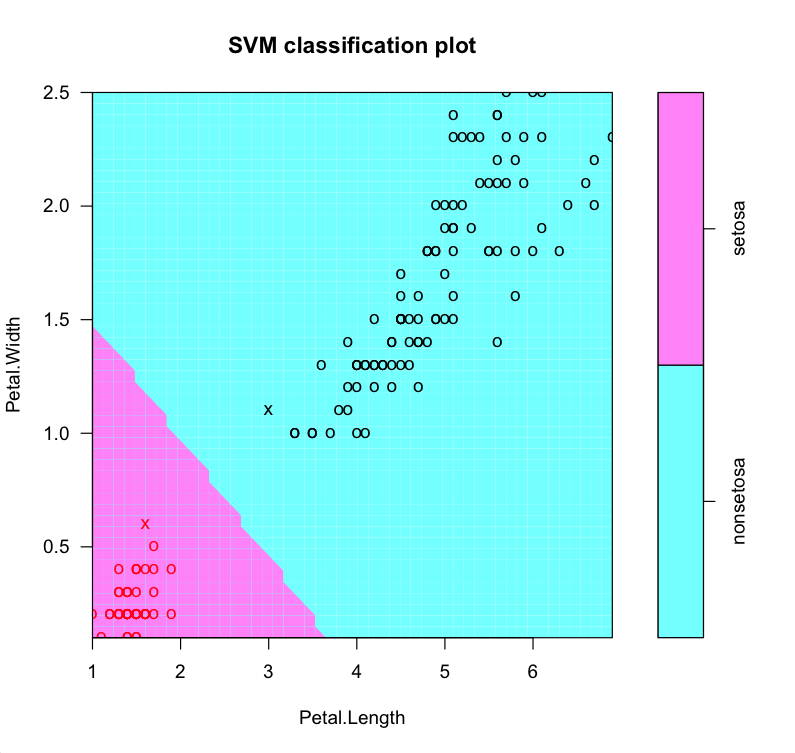
\includegraphics[scale=0.35]{petal_svm}
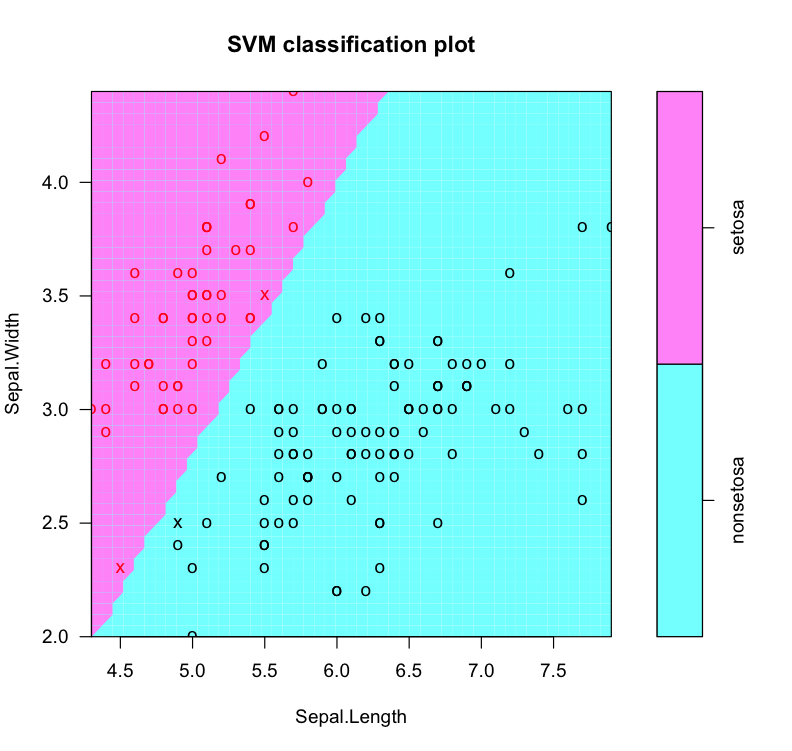
\includegraphics[scale=0.35]{sepal_svm}
\end{center}

\item 1c Is the data set linearly seperable? 

The data is linearly separable in each case.  

\item How many support vectors are there? 

For the petal model, there are 2 support vectors. For the sepal model, there are 3. 

\item Fnd the parameters w and b that define the decision boundary

For the  petal model, w = $    -1.497422,   -1.238551$, b = -1.804382.

For the  petal model, w = $    -7.095041,    3.112485$, b = -5.102501.

%
%w:  -0.4402915   0.3329121   -0.8948921  -0.9260634
%
%b:  -1.474086
  \end{enumerate}
  \item Split \verb|wdbc.data| into 70\% training and 30\% test data
  
    \begin{Verbatim}
    wdbc <- read.table("~/Dropbox/Tarleton/data_mining/dfiles/wdbc.data", 
            header = FALSE, sep = ",")
    wdbc <- wdbc[,-1]
    splitset <- splitdata(wdbc, 0.7, FALSE)
    train <- splitset$train
    \end{Verbatim}
  
  \begin{enumerate}
  \item Fit an SVM to the training data.
  
  \verb|wdbcmodel <- svm(V2~., wdbc[train,])|
  
  \item What type of kernel was used? 
  
  radial
  
  \item Find the classification accuracy of this SVM on the training and test data
  
  test accuracy: 97.07602\%
  
  train accuracy: 98.49246\%
  
  The confusionmatrix for the train accuracy is 
  $$
  \begin{matrix}
   & B &   M \\
   B & 240 &   1\\
   M &   5 & 152
  \end{matrix}
  $$
  
  \item Use the tune.svm command to tune the values of cost and $\gamma$. It may 
   take some experimentation to find suitable ranges for these parameters. 
  \begin{Verbatim}
  ogamma <- wdbcmodel$gamma
  ocost <- wdbcmodel$cost
  tunewdbc <- tune.svm(V2~., data=wdbc[train,], 
                       gamma=10^(-4:1), cost=10^(-1:2))
  
  ngamma <- (tunewdbc$best.parameters)[1]
  ncost <- (tunewdbc$best.parameters)[2]
  \end{Verbatim}

  The original values for $\gamma$ and cost were $0.0\bar{3}$ and 1 respectively. 
  After tuning, the best values were 0.01 and 1 respectively. 
  
  \item Refit the SVM using the tuned cost and gamma values
  \begin{Verbatim}
  wdbcmodel2 <- svm(V2~., data=wdbc[train,],gamma=ngamma,cost=ncost)
  predwdbc2 <- predict(wdbcmodel2, newdata = wdbc[-train,])
  confmatrix(wdbc$V2[-train], predwdbc2)
  \end{Verbatim}

  \item Find the classification accuracy of the tuned SVM on the training 
     and test data
  
   test accuracy: 95.32164\%

   train accuracy: 98.49246\%

   The confusion matrix for the train accuracy is 
   $$
   \begin{matrix}
       & B &   M  \\ 
       B & 241 &   0\\
       M &   6 & 151
   \end{matrix}
   $$
   At a glance, it can be seen that the accuracy for the predicted values on the 
   test set actually decreased with the tuned values. This is most likely due to 
   overfitting, since the training set did not show decreased accuracy. 
\end{enumerate}
\item
Create a data set similar to the one below, where there are four 
normally distributed clusters, each containing 50 points, centered at 
$$
                 (0, 0), (0, 6), (6, 0), (6, 6)
$$
for all four clusters, $\sigma_x = \sigma_y = 1.5$.
  \begin{Verbatim}
  bcx <- rnorm(50, 0, 1.5)
  bcy <- rnorm(50, 0, 1.5)
  bcx <- c(bcx, rnorm(50, 6, 1.5))
  bcy <- c(bcy, rnorm(50, 6, 1.5))
  
  rtx <- rnorm(50, 6, 1.5)
  rty <- rnorm(50, 0, 1.5)
  rtx <- c(rtx, rnorm(50, 0, 1.5))
  rty <- c(rty, rnorm(50, 6, 1.5))
  
  x <- c(bcx, rtx)
  y <- c(bcy, rty)
  type <- rep('square', 100)
  type <- c(type, rep('triangle', 100))
  
  plot(bcx, bcy, type='p',col='blue', pch = 15)
  lines(rtx, rty, type='p',col='green', pch=17)
  
  points <- data.frame(x = x, y = y, type = type)
  \end{Verbatim}
\item Create an SVM for distinguishing between the blue and green nodes, plot the 
  SVM, and calculate its classification accuracy.
\begin{center}
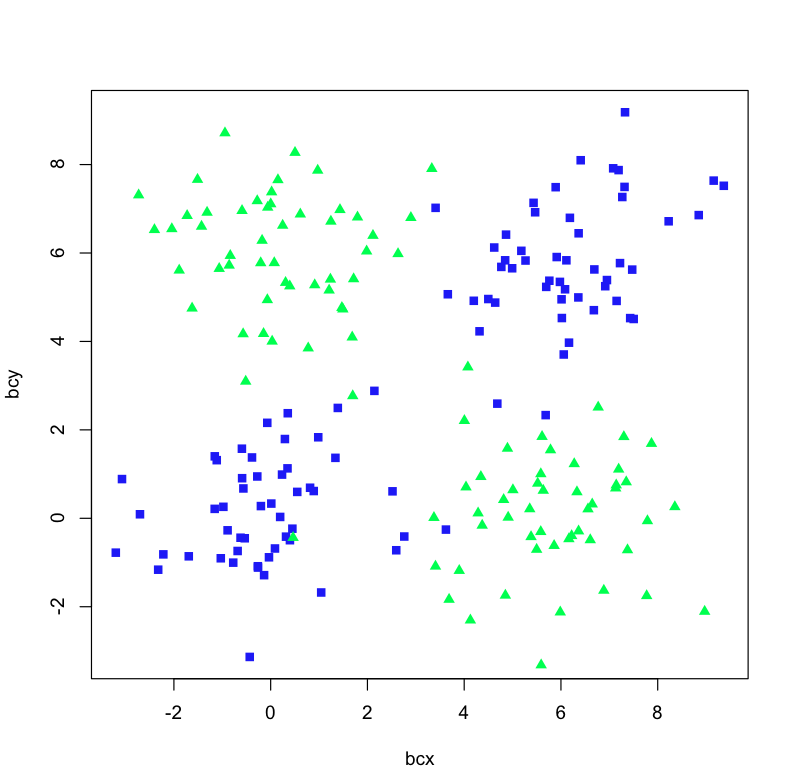
\includegraphics[scale=0.35]{points}
\end{center}

\begin{center}
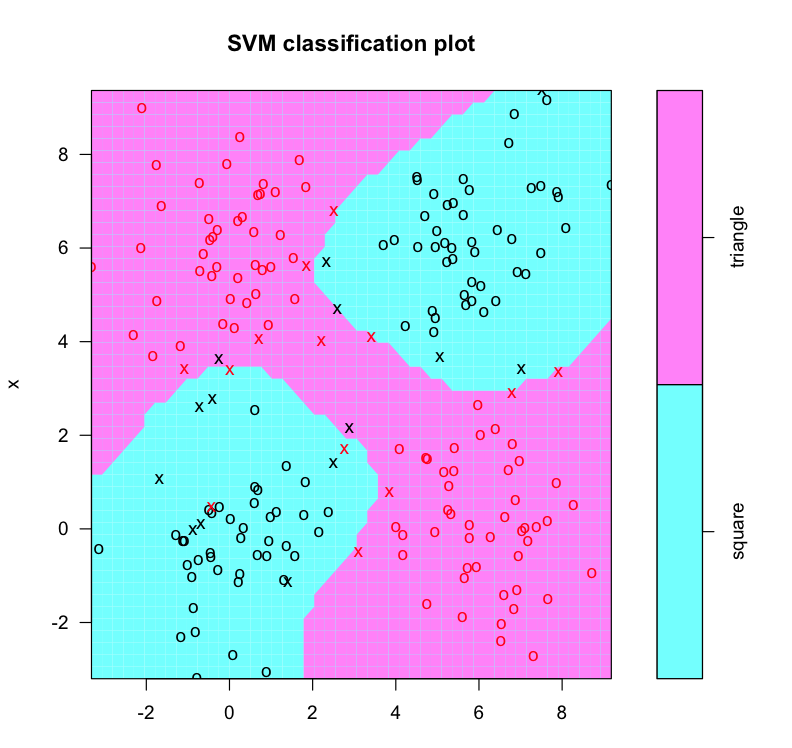
\includegraphics[scale=0.35]{svmpoints}
\end{center}

The classification accuracy is 97\%

The confusion matrix is 
$$
\begin{matrix}
&       square & triangle \\
  square    &   97  &       3 \\
  triangle  &    3  &     97
\end{matrix}
$$
\end{enumerate}


\begin{Verbatim}
#Data Mining Hw 12
library(e1071)
#1a. Create a version of the iris data set, where the class labels 
#    "versicolor" and "virginica" are replaced by "nonsetosa". This 
#    problem involves building an SVM to classify iris flowers as 
#    setosa or nonsetosa

new_iris <- iris
idx <- (new_iris$Species == 'setosa') * 1
Species <- rep('',length(idx))
Species[idx == 1] <- 'setosa'
Species[idx != 1] <- 'nonsetosa'
new_iris$Species <- Species
levels(new_iris$Species) <- c('setosa', 'nonsetosa')

# 1b Fit a linear support vector machine to the data with cost = 1000 
#    and plot the SVM

#Separate model for comparison
petalmodel <- svm(as.factor(Species)~Petal.Length + Petal.Width, 
                  new_iris, kernel='linear',cost=1000)
plot(petalmodel, new_iris, Petal.Width~Petal.Length, )

sepalmodel <- svm(as.factor(Species)~Sepal.Length + Sepal.Width, 
                  new_iris, kernel='linear',cost=1000)
plot(sepalmodel, new_iris, Sepal.Width~Sepal.Length, )

speciesmodel <- svm(as.factor(Species)~., new_iris, kernel='linear',cost = 1000)
plot(speciesmodel, new_iris, Petal.Width~Petal.Length)

# 1c Is the data set linearly seperable? 

# 1d How many support vectors are there? 
sum(speciesmodel$nSV)

#1e Fnd the parameters w and b that define the decision boundary
w = t(speciesmodel$coefs) %*% (speciesmodel$SV)
b = -speciesmodel$rho

#2 Split wdbc.data into 70% training and 30% test data

wdbc <- read.table("~/Dropbox/Tarleton/data_mining/dfiles/wdbc.data", 
        header = FALSE, sep = ",")
wdbc <- wdbc[,-1]
splitset <- splitdata(wdbc, 0.7, FALSE)
train <- splitset$train

#2a Fit an SVM to the training data.

wdbcmodel <- svm(V2~., wdbc[train,])

#2b What type of kernel was used? 

#2c Find the classification accuracy of this SVM on the training and test data
predwdbc <- predict(wdbcmodel, newdata = wdbc[-train,])
predwdbc <- predict(wdbcmodel, newdata = wdbc[train,])
confmatrix(wdbc$V2[train], predwdbc)

#2d Use the tune.svm command to tune the values of cost and gamma. It may 
#   take some experimentation to find suitable ranges for these parameters. 
ogamma <- wdbcmodel$gamma
ocost <- wdbcmodel$cost
tunewdbc <- tune.svm(V2~., data=wdbc[train,], gamma=10^(-4:1), cost=10^(-1:2))

ngamma <- (tunewdbc$best.parameters)[1]
ncost <- (tunewdbc$best.parameters)[2]

#2e Refit the SVM using the tuned cost and gamma values
wdbcmodel2 <- svm(V2~., data=wdbc[train,],gamma=ngamma,cost=ncost)
predwdbc2 <- predict(wdbcmodel2, newdata = wdbc[-train,])
confmatrix(wdbc$V2[-train], predwdbc2)

#2f Find the classification accuracy of the tuned SVM on the training 
#   and test data


#3a Create a data set similar to the one below, where there are four 
#   normally distributed clusters, each containing 50 points, centered at 
#                    (0, 0), (0, 6), (6, 0), (6, 6)
#   for all four clusters, sigma_x = sigma_y = 1.5.
bcx <- rnorm(50, 0, 1.5)
bcy <- rnorm(50, 0, 1.5)
bcx <- c(bcx, rnorm(50, 6, 1.5))
bcy <- c(bcy, rnorm(50, 6, 1.5))

rtx <- rnorm(50, 6, 1.5)
rty <- rnorm(50, 0, 1.5)
rtx <- c(rtx, rnorm(50, 0, 1.5))
rty <- c(rty, rnorm(50, 6, 1.5))

x <- c(bcx, rtx)
y <- c(bcy, rty)
type <- rep('square', 100)
type <- c(type, rep('triangle', 100))

plot(bcx, bcy, type='p',col='blue', pch = 15)
lines(rtx, rty, type='p',col='green', pch=17)

points <- data.frame(x = x, y = y, type = type)
#3b Create an SVM for distinguishing between the blue and green nodes, plot the 
#   SVM, and calculate its classification accuracy.
pointmodel <- svm(as.factor(type)~., points, cost=1000)
plot(pointmodel, points)
predpoint <- predict(pointmodel, newdata = points)
confmatrix(points$type, predpoint)

\end{Verbatim} 

\end{document}
